\documentclass[journal]{IEEEtran}

\usepackage{blindtext}
\usepackage{cite}
\usepackage{graphicx}
\usepackage{array}
\usepackage{color}
\usepackage{tabularx}
\usepackage{epsfig}
\usepackage{amsmath}
\usepackage{amssymb}
\usepackage{bm}
\usepackage{wasysym}
\usepackage{circuitikz}
\usepackage{float}
\usepackage{algorithm}
\usepackage{algorithmic}

\usetikzlibrary{arrows,shapes,calc,positioning}

\newcommand{\myscope}[2]
{\draw[thick,rotate=#2] (#1) circle (12pt)
(#1) ++(-0.35,-0.1) --++ (0.3,0.3) --++ (0,-0.3) --++(0.3,0.3) --++(0,-0.3);}

\begin{document}

\title{CSCE 221 \\ Problem Set 18}

\author{Jacob~Purcell,~\IEEEmember{Texas~A\&M,~Student}}

\maketitle
\section{}
\subsection{}
\begin{figure}[h!]
    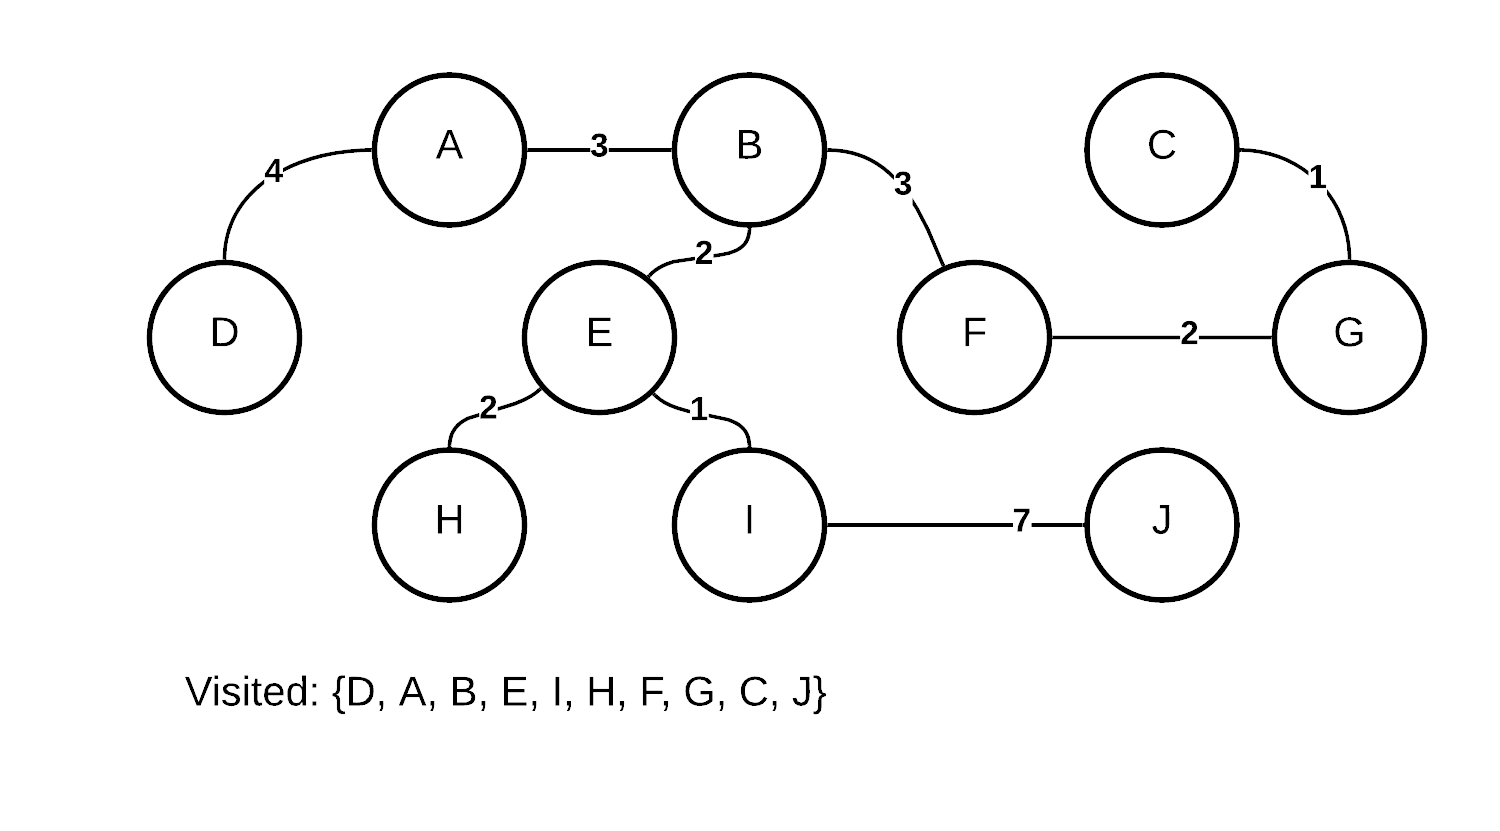
\includegraphics[scale = 0.17]{pa.png}
    \caption{Minimum spanning tree generated by Prim's Algorithm.}
\end{figure}

\subsection{}
\begin{figure}[h!]
    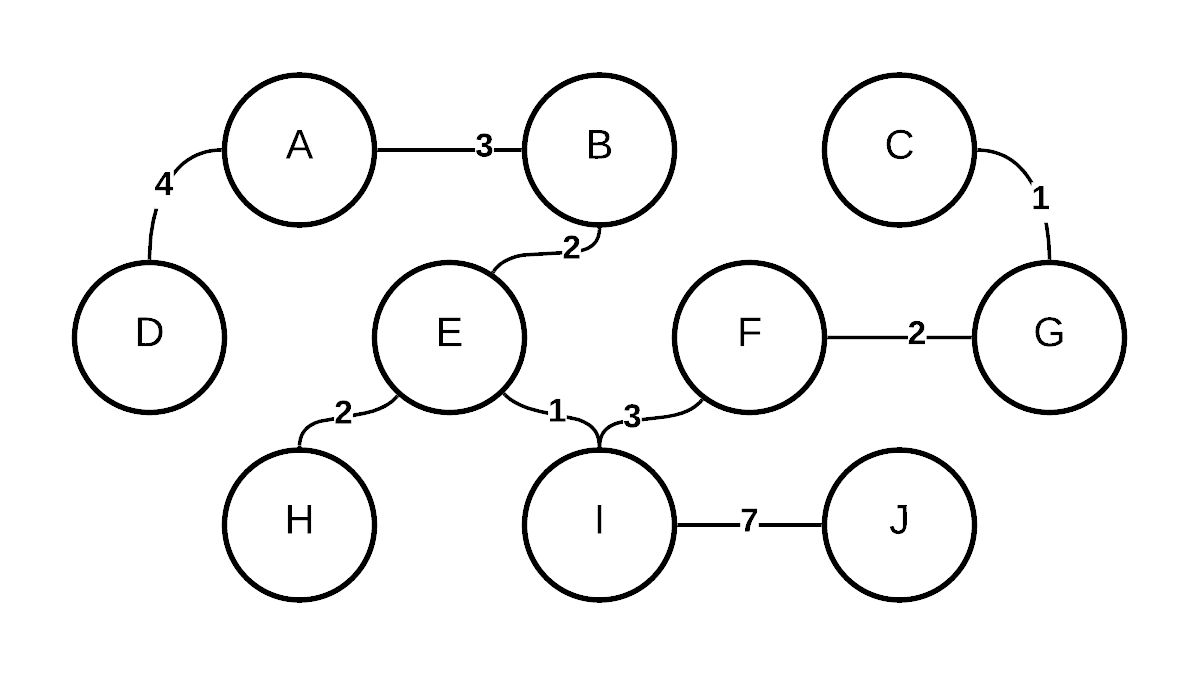
\includegraphics[scale = 0.17]{ka.png}
    \caption{Minimum spanning tree generated by Kruskal's Algorithm.}
\end{figure}

\subsection{}
These trees are not unique as there are arbitrary choices in both algorithms that may 
result in the same minimum spanning tree.

\section{}
Using Cayley's formula 
$$n^{n-2}$$
where n is the number of vertices,

\subsection{}
$$1^{-1} = \boxed{1}$$

\subsection{}
$$2^0 = \boxed{1}$$

\subsection{}
$$3^1 = \boxed{3}$$

\subsection{}
$$4^2 = \boxed{16}$$

\subsection{}
The number of unrooted trees will be $T$. For any $T$, there are $V$ possible root nodes,

$$TV$$

For any root node there are $(V-1)!$ edge configurations

$$TV(V-1)!$$
$$TV!$$

At the same time, if we add edges one by one to the nodes, we have $V(V-1)$ possible places, then
$V(V-2)$ and so on, which yields the possible number of trees,

$$\Pi_{k=1}^{V} V(k-1) = V^{V-2}V!$$

$$TV! = V^{V-2}V!$$
$$T = \boxed{V^{V-2}}$$

\end{document}
